\documentclass[a4paper]{scrartcl}
\usepackage{amsmath}
\usepackage{amsfonts}
\usepackage{amssymb}
\usepackage[utf8]{inputenc}
\usepackage[frenchb]{babel}
\usepackage[T1]{fontenc}
\usepackage{lmodern}
\usepackage{graphicx}

\title{Implémentation d'un moteur physique 2D dans un langage fonctionnel}
\subtitle{Et plus encore...}

\begin{document}
\maketitle

\tableofcontents

\newpage

\section*{Introduction}
\addcontentsline{toc}{section}{Introduction}

\section{Philosophie de développement et organisation du code}
\paragraph{Un moteur purement fonctionnel}

[comment ça marche ? on a des fonctions world -> world et avec >>= on
a une syntaxe cool]
\paragraph{Les modules pour hiérarchiser, organiser le code et
  abstraire les implémentations}
\begin{figure}[h]
  \centering
  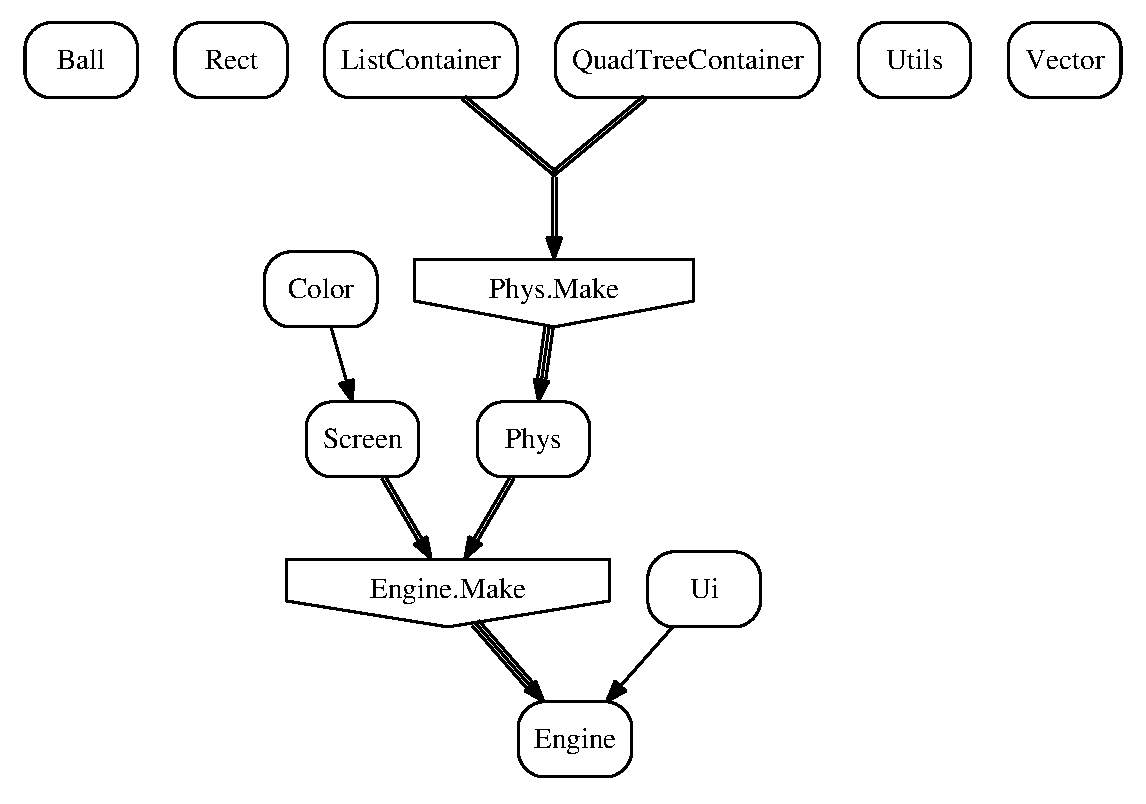
\includegraphics[scale = 0.7]{modules.eps}  
  \caption{Architecture des modules composant le projet}
  \label{fig:modules}
\end{figure}

\paragraph{Un moteur généraliste et réutilisable}

\section*{}
À présent, il est temps de regarder de plus près les implémentations
effectives des modules présentés. Au programme : structures de données
fonctionnelles, simulation physique et gestion des collisions.

\section{Containeurs de balles : les modules \texttt{ListContainer}
  et \texttt{QuadTreeContainer}}
\subsection{Structures de données fonctionnelles et \emph{Zippers}}
\subsection{\texttt{ListContainer} : conteneurs utilisant des listes}
\subsection{\texttt{QuadTreeContainer} : une structure arborescente
  pour stocker nos balles}

\section{Simulation physique : module \texttt{Phys}}
[module Phys obtenu comme image du foncteur Phys.Make sur un module
conteneur]
\subsection{Monde physique, objets physique : simulation simple sans
  collisions}
\subsection{Gestion des collisions}
\paragraph{Un peu de physique}
\paragraph{En pratique}
\subsection{Ce que nous permettrait également notre monde purement
  fonctionnel}
[Gestion plus fine des collisions, backtrack / dichotomie]

\section*{}
On a maintenant un moteur physique 2D (ne gérant certes que des
balles), prenant en compte des forces, des collisions, et pouvant
s'utiliser de manière totalement indépendante. Il fournit un monde
physique (\texttt{Phys.world}) dans lequel on peut ajouter des balles,
des forces, … et dont on peut ensuite simuler l'évolution.

Ainsi, en vertu du sacro-saint principe d'isolement, ce module ne
traite pas avec l'affichage. Son rôle est simplement de simuler la
physique.

Et c'est parce que l'on veut quand même pouvoir afficher des choses à
l'écran qu'intervient...

\section{Le module \texttt{Engine} : un moteur de jeu}

[ce qu'on appelle moteur de jeu est en réalité un module gérant tout
ce qui touche à la physique, l'affichage, et qui permet à
l'utilisateur de programmer aisément des situations variées]



Le module Engine est le module avec lequel traitera au final
l'utilisateur : il doit principalement permettre de simuler la
physique et fournir une sortie graphique quelconque. Son rôle est en
fait d'agencer les deux mondes : «~brancher~» le moteur physique, qui
ne connait rien de l'affichage, sur un module dédié à l'affichage, qui
lui ne connait rien des objets physiques.

La pièce centrale d'\texttt{Engine} est donc une fois encore un
foncteur, \texttt{Make}, prenant en argument un module contenant un
moteur physique (\texttt{Phys}, par exemple) et un autre module
fournissant une sortie graphique.

Nous avons ici implémenté un module \texttt{Screen} ayant ce rôle,
mais il est tout à fait possible (hypothétiquement) d'écrire un module
réalisant par exemple la sortie graphique dans une vidéo

\subsection{Module \texttt{Screen} : affichage à l'écran}
Le module \texttt{Screen} est une implémentation satisfaisant la
signature qu'\texttt{Engine.Make} attend pour un module
d'affichage. Il permet ainsi d'abstraire l'utilisation du module
\texttt{Graphics}, lui même place d'un joyeux bazar puisqu'il condense
plein de fonctionnalités a priori sans rapport.

Le contenu de \texttt{Screen} est en pratique peu intéressant,
puisqu'il ne s'agit que d'une surcouche aux fonctions de dessin de
\texttt{Graphics}. Il définit un buffer d'affichage, contenant la
taille de l'écran et des informations spécifiques à l'implémentations
(cachées dans un type abstrait par la signature), comme le
\emph{double buffering} (activé).

\subsection{Que fait exactement \texttt{Engine} ?}
\texttt{Engine}


\end{document}
